
\section{Integration algorithms}
\label{integration}

\subsection{The Verlet Algorithms}

DL\_POLY integration algorithms\index{algorithm} are based on 
the Verlet\index{algorithm!Verlet}
scheme, which is both time reversible and simple \cite{allen-89a}. 
It generates trajectories in the
microcanonical (NVE) ensemble in which the total energy (kinetic plus
potential energy) is conserved. If this property drifts or fluctuates
excessively in the course of a simulation it indicates that the
timestep is too large or the potential cutoffs too small (relative
r.m.s. fluctuations in the total energy of $10^{-5}$ are typical with
this algorithm).

\D{} contains two versions of the Verlet algorithm. The first is the Verlet
leapfrog\index{algorithm!Verlet leapfrog} (LF) algorithm and the second is
the velocity Verlet\index{algorithm!velocity Verlet} (VV). 

\subsubsection{Verlet Leapfrog}
The LF algorithm requires values of position $(\vek{r}$) and force
($\vek{f}$) at time $t$ while the velocities ($\vek{v}$) are half a
timestep behind. The first step is to advance the velocities to
$t+(1/2)\Delta t$ by integration of the force:
\begin{equation}
\vek{v}(t + {1\over 2} \Delta t) \leftarrow  \vek{v}(t-{1\over 2} \Delta t) + \Delta t \; {\vek{f}(t)\over m}
\end{equation}
where $m$ is the mass of a site and $\Delta t$ is the timestep.

The positions are then advanced using the new velocities:
\begin{equation}
\vek{r}(t+\Delta t) \leftarrow \vek{r}(t) + \Delta t \;\vek{v}(t+{1\over 2}\Delta t)
\end{equation}

Molecular dynamics simulations normally require properties that depend
on position and velocity {\em at the same time} (such as the sum of
potential and kinetic energy).  In the LF algorithm the velocity at
time $t$ is obtained from the average of the velocities half a
timestep either side of time $t$:
\begin{equation}
\vek{v}(t) = {1\over 2} \left[\vek{v}(t-{1\over 2}\Delta t) + \vek{v}(t+{1\over 2}\Delta t)\right]
\end{equation}

The full selection of LF integration algorithms within \D{} is
as follows:

\begin{tabbing}
XXXXXX\=XXXXXXXXXXXXXXXXXXXXXXXXXXXXXXXXXXXXXXXXXXXXXXXXXXXX\kill\\
{\sc nve\_1}    \>  Verlet\index{algorithm!Verlet leapfrog} leaprog with SHAKE\index{algorithm!SHAKE} \\
{\sc nveq\_1}   \>  Rigid units with FIQA\index{algorithm!FIQA} and SHAKE\index{algorithm!SHAKE}\\
{\sc nveq\_2}   \>  Linked rigid units with QSHAKE\index{algorithm!QSHAKE} \\
{\sc nvt\_b1}   \>  Constant T\index{ensemble!Berendsen NVT} (Berendsen \cite{berendsen-84a}) with SHAKE\index{algorithm!SHAKE} \\
{\sc nvt\_e1}   \>  Constant T\index{ensemble!Evans NVT} (Evans \cite{evans-84a}) with SHAKE\index{algorithm!SHAKE} \\
{\sc nvt\_h1}   \>  Constant T\index{ensemble!Hoover NVT} (Hoover \cite{hoover-85a}) with SHAKE\index{algorithm!SHAKE} \\
{\sc nvtq\_b1}  \>  Constant T\index{ensemble!Berendsen NVT} (Berendsen \cite{berendsen-84a}) with FIQA\index{algorithm!FIQA} and SHAKE\index{algorithm!SHAKE} \\
{\sc nvtq\_b2}  \>  Constant T\index{ensemble!Berendsen NVT} (Berendsen \cite{berendsen-84a}) with QSHAKE\index{algorithm!QSHAKE} \\
{\sc nvtq\_h1}  \>  Constant T\index{ensemble!Hoover NVT} (Hoover \cite{hoover-85a}) with FIQA\index{algorithm!FIQA} and SHAKE\index{algorithm!SHAKE} \\
{\sc nvtq\_h2}  \>  Constant T\index{ensemble!Hoover NVT} (Hoover \cite{hoover-85a}) with QSHAKE\index{algorithm!QSHAKE} \\
{\sc npt\_b1}   \>  Constant T,P\index{ensemble!Berendsen NPT} (Berendsen \cite{berendsen-84a}) with FIQA\index{algorithm!FIQA} and SHAKE\index{algorithm!SHAKE} \\
{\sc npt\_h1}   \>  Constant T,P+\index{ensemble!Hoover NPT} (Hoover \cite{hoover-85a}) with SHAKE\index{algorithm!SHAKE} \\
{\sc nptq\_b1}  \>  Constant T,P\index{ensemble!Berendsen NPT} (Berendsen \cite{berendsen-84a}) with FIQA\index{algorithm!FIQA} and SHAKE\index{algorithm!SHAKE}\\
{\sc nptq\_b2}  \>  Constant T,P\index{ensemble!Berendsen NPT} (Berendsen \cite{berendsen-84a}) with QSHAKE\index{algorithm!QSHAKE} \\
{\sc nptq\_h1}  \>  Constant T,P\index{ensemble!Hoover NPT} (Hoover \cite{hoover-85a}) with FIQA\index{algorithm!FIQA} and SHAKE\index{algorithm!SHAKE}\\
{\sc nptq\_h2}  \>  Constant T,P\index{ensemble!Hoover NPT} (Hoover \cite{hoover-85a}) with QSHAKE\index{algorithm!QSHAKE} \\
{\sc nst\_b1}   \>  Constant T,\mat{\sigma}\index{ensemble!Berendsen N$\sigma$T} (Berendsen \cite{berendsen-84a}) with SHAKE\index{algorithm!SHAKE} \\
{\sc nst\_h1}   \>  Constant T,\mat{\sigma}\index{ensemble!Hoover N$\sigma$T} (Hoover \cite{hoover-85a}) with SHAKE\index{algorithm!SHAKE} \\
{\sc nstq\_b1}  \>  Constant T,\mat{\sigma}\index{ensemble!Berendsen
N$\sigma$T} (Berendsen \cite{berendsen-84a}) with FIQA\index{algorithm!FIQA} and SHAKE\index{algorithm!SHAKE}\\
{\sc nstq\_b2}  \>  Constant T,\mat{\sigma}\index{ensemble!Berendsen N$\sigma$T} (Berendsen \cite{berendsen-84a}) with QSHAKE\index{algorithm!QSHAKE} \\
{\sc nstq\_h1}  \>  Constant T,\mat{\sigma}\index{ensemble!Hoover N$\sigma$T} (Hoover \cite{hoover-85a}) with
FIQA\index{algorithm!FIQA} and SHAKE\index{algorithm!SHAKE}\\
{\sc nstq\_h2}  \>  Constant T,\mat{\sigma}\index{ensemble!Hoover N$\sigma$T} (Hoover \cite{hoover-85a}) with QSHAKE\index{algorithm!QSHAKE} \\
\end{tabbing}
In the above table the FIQA\index{algorithm!FIQA} algorithm is Fincham's Implicit Quaternion\index{quaternions}
Algorithm \cite{fincham-92a} and QSHAKE\index{algorithm!QSHAKE} is the \D{} algorithm combining
rigid bonds and rigid bodies\index{rigid body} in the same molecule \cite{forester-96a}.

\subsubsection{Velocity Verlet}

The VV algorithm assumes that positions, velocities and forces are
known at each full timestep. The algorithm proceeds in two stages as
follows.

In the first stage a half step velocity is calculated: 
\begin{equation}
\vek{v}(t + \frac{1}{2}\Delta t) \leftarrow  \vek{v}(t) + \frac{1}{2}\Delta t \; {\vek{f}(t)\over m}
\end{equation}
and then the full timestep position is obtained:
\begin{equation}
\vek{r}(t+\Delta t) \leftarrow \vek{r}(t) + \Delta t \;\vek{v}(t+{1\over 2}\Delta t)
\end{equation}
In the second stage, using the new positions, the next update of the
forces $f(t+\Delta t)$ is obtained, from which the full step
velocity is calculated using:
\begin{equation}
\vek{v}(t + \Delta t) \leftarrow  \vek{v}(t+{1\over 2} \Delta t) +
{1\over 2} \Delta t \; {\vek{f}(t + \Delta t)\over m}
\end{equation}
Thus at the end of the two stages full synchronisation of the
positions, forces and velocities is obtained.

The full selection of VV integration algorithms within \D{} is
as follows:

\begin{tabbing}
XXXXXXXXX\=XXXXXXXXXXXXXXXXXXXXXXXXXXXXXXXXXXXXXXXXXXXXXXXX\kill\\
{\sc nvevv\_1}    \>  Velocity Verlet\index{algorithm!velocity Verlet} with RATTLE\index{algorithm!RATTLE} \\
{\sc nveqvv\_1}   \>  Rigid units with NOSQUISH\index{algorithm!NOSQUISH} and RATTLE\index{algorithm!RATTLE}\\
{\sc nveqvv\_2}   \>  Linked rigid units with QSHAKE\index{algorithm!QSHAKE} \\
{\sc nvtvv\_b1}   \>  Constant T\index{ensemble!Berendsen NVT} (Berendsen \cite{berendsen-84a}) with RATTLE\index{algorithm!RATTLE} \\
{\sc nvtvv\_e1}   \>  Constant T\index{ensemble!Evans NVT} (Evans \cite{evans-84a}) with RATTLE\index{algorithm!RATTLE} \\
{\sc nvtvv\_h1}   \>  Constant T\index{ensemble!Hoover NVT} (Hoover \cite{hoover-85a}) with RATTLE\index{algorithm!RATTLE} \\
{\sc nvtqvv\_b1}  \>  Constant T\index{ensemble!Berendsen NVT} (Berendsen \cite{berendsen-84a}) with NOSQUISH\index{algorithm!NOSQUISH} and RATTLE\index{algorithm!RATTLE} \\
{\sc nvtqvv\_b2}  \>  Constant T\index{ensemble!Berendsen NVT} (Berendsen \cite{berendsen-84a}) with QSHAKE\index{algorithm!QSHAKE} \\
{\sc nvtqvv\_h1}  \>  Constant T\index{ensemble!Hoover NVT} (Hoover \cite{hoover-85a}) with NOSQUISH\index{algorithm!NOSQUISH} and RATTLE\index{algorithm!RATTLE} \\
{\sc nvtqvv\_h2}  \>  Constant T\index{ensemble!Hoover NVT} (Hoover \cite{hoover-85a}) with QSHAKE\index{algorithm!QSHAKE} \\
{\sc nptvv\_b1}   \>  Constant T,P\index{ensemble!Berendsen NPT} (Berendsen \cite{berendsen-84a}) with NOSQUISH\index{algorithm!NOSQUISH} and RATTLE\index{algorithm!RATTLE} \\
{\sc nptvv\_h1}   \>  Constant T,P+\index{ensemble!Hoover NPT} (Hoover \cite{hoover-85a}) with RATTLE\index{algorithm!RATTLE} \\
{\sc nptqvv\_b1}  \>  Constant T,P\index{ensemble!Berendsen NPT} (Berendsen \cite{berendsen-84a}) with NOSQUISH\index{algorithm!NOSQUISH} and RATTLE\index{algorithm!RATTLE}\\
{\sc nptqvv\_b2}  \>  Constant T,P\index{ensemble!Berendsen NPT} (Berendsen \cite{berendsen-84a}) with QSHAKE\index{algorithm!QSHAKE} \\
{\sc nptqvv\_h1}  \>  Constant T,P\index{ensemble!Hoover NPT} (Hoover \cite{hoover-85a}) with NOSQUISH\index{algorithm!NOSQUISH} and RATTLE\index{algorithm!RATTLE}\\
{\sc nptqvv\_h2}  \>  Constant T,P\index{ensemble!Hoover NPT} (Hoover \cite{hoover-85a}) with QSHAKE\index{algorithm!QSHAKE} \\
{\sc nstvv\_b1}   \>  Constant T,\mat{\sigma}\index{ensemble!Berendsen N$\sigma$T} (Berendsen \cite{berendsen-84a}) with RATTLE\index{algorithm!RATTLE} \\
{\sc nstvv\_h1}   \>  Constant T,\mat{\sigma}\index{ensemble!Hoover N$\sigma$T} (Hoover \cite{hoover-85a}) with RATTLE\index{algorithm!RATTLE} \\
{\sc nstqvv\_b1}  \>  Constant T,\mat{\sigma}\index{ensemble!Berendsen
N$\sigma$T} (Berendsen \cite{berendsen-84a}) with NOSQUISH\index{algorithm!NOSQUISH} and RATTLE\index{algorithm!RATTLE}\\
{\sc nstqvv\_b2}  \>  Constant T,\mat{\sigma}\index{ensemble!Berendsen N$\sigma$T} (Berendsen \cite{berendsen-84a}) with QSHAKE\index{algorithm!QSHAKE} \\
{\sc nstqvv\_h1}  \>  Constant T,\mat{\sigma}\index{ensemble!Hoover N$\sigma$T} (Hoover \cite{hoover-85a}) with
NOSQUISH\index{algorithm!NOSQUISH} and RATTLE\index{algorithm!RATTLE}\\
{\sc nstqvv\_h2}  \>  Constant T,\mat{\sigma}\index{ensemble!Hoover N$\sigma$T} (Hoover \cite{hoover-85a}) with QSHAKE\index{algorithm!QSHAKE} \\
\end{tabbing}

In the above table the NOSQUISH\index{algorithm!NOSQUISH} algorithm is
the rotational algorithm of Miller {\em et al} \cite{miller-02a} and
QSHAKE\index{algorithm!QSHAKE} is the \D{} algorithm combining rigid
bonds and rigid bodies\index{rigid body} in the same molecule
\cite{forester-96a}.

\subsubsection{Temperature and Energy Conservation}

For both VV and LF the instantaneous temperature can be obtained
from the atomic velocities assuming the system has no net momentum:
\begin{equation}
{\cal  T} = {\sum_{i=1}^{\cal N} m_i v^2_i(t) \over  k_B f} 
\end{equation}
where $i$ labels particles (which can be atoms or rigid molecules),
${\cal N}$ the number of particles in the system, $k_B$ Boltzmanns
constant and $f$ the number of degrees of freedom in the system
($3{\cal N} - 3$ if the system is periodic and without constraints).

The total energy of the system is a conserved quantity
\begin{equation}
{\cal H}_{\rm NVE} = U + KE
\end{equation}
where $U$ is the potential energy of the system and $KE$ the kinetic energy at time $t$.

\subsection{Bond Constraints}

\subsubsection{SHAKE}
\label{shake}

The SHAKE algorithm for bond constraints was devised by Ryckaert {\em
et al.} \cite{ryckaert-77a} and is based on the Verlet leapfrog
\index{algorithm!Verlet leapfrog} integration scheme
\cite{allen-89a}. It is a two stage scheme. In the first stage the
leapfrog algorithm calculates the motion of the atoms in the system
assuming a complete absence of the rigid bond\index{rigid
bond|see{constraints,bond}} forces. The positions of the atoms at the
end of this stage do not conserve the distance constraint required by
the rigid bond\index{rigid body} and a correction is necessary.  In
the second stage the deviation in the length of a given rigid
bond\index{constraints!bond} is used retrospectively to compute the
constraint force needed to conserve the bondlength.  It is relatively
simple to show that the constraint force has the form
\begin{equation}
\vek{G}_{ij}\approx\frac{\mu_{ij}(d_{ij}^{2}-d_{ij}'^{2})}
{2\Delta t^{2}\vek{d}_{ij}^{o}\cdot\vek{d}_{ij}'}\vek{d}_{ij}^{o} \label{g12}
\end{equation}
where:~$\mu_{ij}$ is the reduced mass of the two atoms connected by
the bond;~$\vek{d}_{ij}^{o}$ and $\vek{d}_{ij}'$ are the original and
intermediate bond vectors; $d_{ij}$ is the constrained bondlength; and
$\Delta t$ is the Verlet\index{algorithm!Verlet} integration timestep. It should be noted
that this formula is an approximation only.

\begin{figure}[ht]
\begin{center}
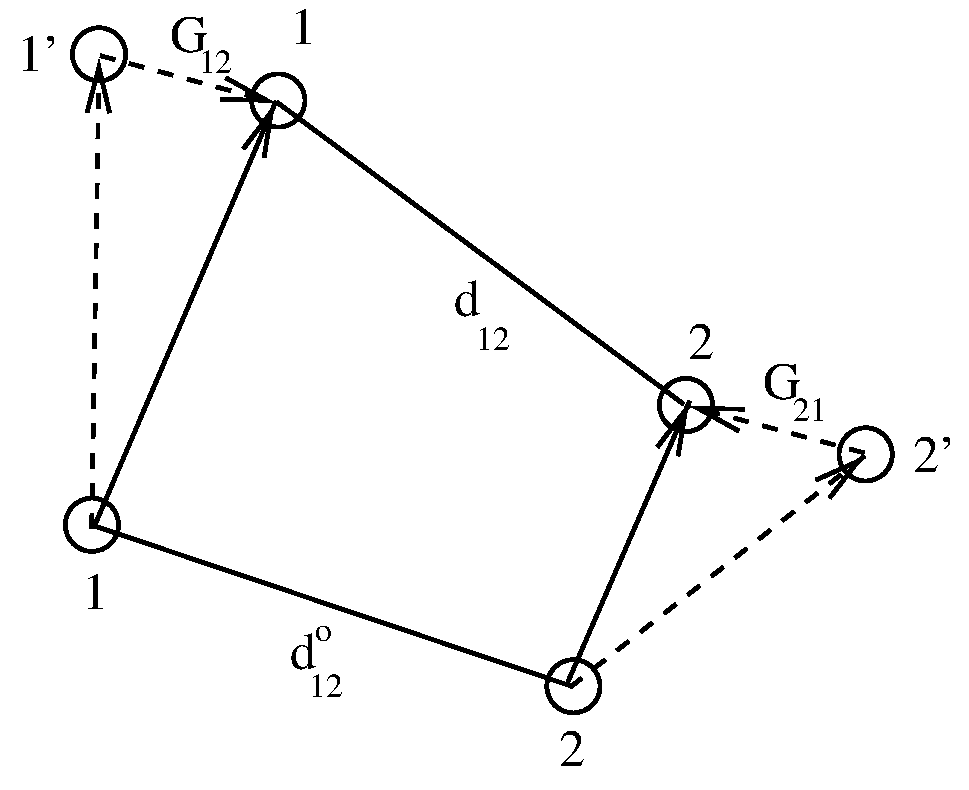
\includegraphics[height=8cm]{shake.eps}
\caption{The SHAKE algorithm}
\end{center}
The algorithm calculates the constraint force
$\vek{G}_{12}=-\vek{G}_{21}$ that conserves the bondlength $d_{12}$
between atoms $1$ and $2$, following the initial movement to positions
$1'$ and $2'$ under the unconstrained forces $\vek{F}_{1}$ and $\vek{F}_{2}$.
\end{figure}

For a system of simple diatomic molecules, computation of the
constraint force will, in principle, allow the correct atomic
positions to be calculated in one pass.  However in the general
polyatomic case this correction is merely an interim adjustment, not
only because the above formula is approximate, but the successive
correction of other bonds in a molecule has the effect of perturbing
previously corrected bonds. The SHAKE algorithm is therfore iterative,
with the correction cycle being repeated for all bonds until each has
converged to the correct length, within a given tolerance.  The
tolerance may be of the order $10^{-4}~\AA$ to $10^{-8}~\AA$ depending
on the precision desired.

The procedure may be summarised as follows:
\begin{enumerate}
\item All atoms in the system are moved using the Verlet\index{algorithm!Verlet} algorithm, 
assuming an absence of rigid bonds\index{constraints!bond} 
(constraint forces).  (This is
stage 1 of the SHAKE algorithm.)
\item The deviation in each bondlength is used to calculate the 
corresponding constraint force (\ref{g12}) that (retrospectively)
`corrects' the bond length.
\item After the correction (\ref{g12}) has been applied to all bonds, every
bondlength is checked. If the largest deviation found exceeds the
desired tolerance, the correction calculation is repeated.
\item Steps 2 and 3 are repeated until all bondlengths satisfy the 
convergence criterion (This iteration constitutes stage 2 of the SHAKE
algorithm).
\end{enumerate}

\D{} implements a parallel version of this algorithm
\cite{smith-94b} (see section \ref{parshake}).  The
subroutine {\sc nve\_1} implements the Verlet
leapfrog\index{algorithm!Verlet} algorithm with bond constraints for
the NVE ensemble. The routine {\sc rdshake\_1} is called to apply the
SHAKE corrections to position.

It should be noted that the fully converged constraint forces
$G_{ij}$ make a contribution to the system virial and the stress
tensor\index{stress tensor}.

The contribution to be added to the atomic virial (for each constrained
bond) is
\begin{equation}
{\cal W}=-\vek{d}_{ij}\cdot\vek{G}_{ij}.
\end{equation}

The contribution to be added to the atomic stress tensor
\index{stress tensor} is given by
\begin{equation}
\sigma^{\alpha \beta}=d_{ij}^{\alpha}G_{ij}^{\beta},
\end{equation}
where $\alpha$ and $\beta$ indicate the $x,y,z$ components. The atomic
stress tensor derived from the pair forces is symmetric.

\subsubsection{RATTLE}
\label{rattle}

RATTLE\index{algorithm!RATTLE} \cite{andersen-83a} is the VV version
of SHAKE. It has two parts: the first constrains the bondlength and
the second adds an additional constaint to the velocities of the atoms
in the constrained bond. The first of these constraints leads to an
expression for the constriant force similar to that for SHAKE:

\begin{equation}
\vek{G}_{ij}\approx\frac{\mu_{ij}(d_{ij}^{2}-d_{ij}'^{2})}
{\Delta t^{2}\vek{d}_{ij}^{o}\cdot\vek{d}_{ij}'}\vek{d}_{ij}^{o} \label{gg12}
\end{equation}

Note that this formula differs from  equation (\ref{g12}) by a factor
of 2. This constraint force is applied during the first stage of the velocity
Verlet algorithm.

The second constraint condition attempts to maintain the relative
velocities of the atoms sharing a bond to a direction perpendicular to
the bond vector. This provides another constraint force:

\begin{equation}
\vek{H}_{ij}\approx-\frac{2\mu_{ij}}{\Delta t}
\frac{\vek{d}_{ij}\cdot(\vek{v}_{j}-\vek{v}_{i})}{\vek{d}_{ij}^{2}}
\vek{d}_{ij}\label{hh12}
\end{equation}

This constraint force is applied during the second stage of the velocity
Verlet algorithm. Both constraint force calculations are iterative and
are brought to convergence before proceeding to the next stage of the
velocity Verlet scheme.

\D{} implements a parallel version of RATTLE that is based on the same
approach as SHAKE \cite{smith-94b} (see section \ref{parshake}).  The
subroutine {\sc nvevv\_1} implements the velocity Verlet
\index{algorithm!velocity Verlet} algorithm with bond constraints in
the NVE ensemble. The subroutine {\sc rdrattle\_r} is called to apply
the corrections to atom positions and the subroutine {\sc rdrattle\_v}
is called to correct the atom velocities.

\subsection{Potential of Mean Force (PMF) Constraints and the Evaluation of Free Energy}
\index{constraints!PMF}\label{PMF}
\index{free energy!potential of mean force|see{constraints!PMF}}

A generalization of bond constraints\index{constraints!bond} can be made to constrain a system
to some point along a reaction coordinate. A simple example of such a
reaction coordinate would be the distance between two ions in
solution. If a number of simulations are conducted with the system
constrained to different points along the reaction coordinate then the
mean constraint force may be plotted as a function of reaction
coordinate and the function integrated to obtain the free energy for
the overall process \cite{mccammon-87a}.  The PMF constraint force,
virial and contributions to the stress tensor are obtained in a manner
analagous to that for a bond constraint\index{constraints!bond} (see previous section). The
only difference is that the constraint is now applied between the
centres of two groups which need not be atoms alone.
\D{} reports the PMF constraint\index{constraints!PMF} virial, {\cal W}, for each simulation. 
Users can convert this to the PMF constraint force from 
\[ G_{\rm PMF} = - {\cal W}_{\rm PMF} / d_{\rm PMF} \]
where $d_{\rm PMF}$ is the constraint distance between the two groups
used to define the reaction coordinate.

\D{} can calculate the PMF using either LF or VV algorithms.
Subroutines {\sc pmflf} and {\sc pmf\_shake} are used in the LF scheme
and subroutines {\sc pmfvv, pmf\_rattle\_r} and {\sc pmf\_rattle\_v}
are used in the VV scheme.

\subsection{Thermostats}

The system may be coupled to a heat bath to ensure that the average
system temperature is maintained close to the requested temperature,
$T_{\rm ext}$. When this is done the equations of motion are modified
and the system no longer samples the microcanonical
ensemble\index{ensemble!NVE}. Instead trajectories in the canonical
(NVT) ensemble\index{ensemble!canonical}, or something close to it are
generated. \D{} comes with three different thermostats: Nos\'e~-Hoover
\cite{hoover-85a}, Berendsen \cite{berendsen-84a}, and Gaussian
constraints\index{constraints!Gaussian} \cite{evans-84a}. Of these
only the Nos\'e-Hoover algorithm generates trajectories in the
canonical (NVT) ensemble. The other methods will produce properties
that typically differ from canonical averages by ${\cal O}(1/{\cal
N})$ \cite{allen-89a}

\subsubsection{Nos\'e~- Hoover Thermostat}

In the Nos\'e-Hoover algorithm \cite{hoover-85a}
Newton's equations of motion are modified to read:
\begin{eqnarray}
{d \vek{r}(t) \over d t}& =& \vek{v}(t)\nonumber \\ {d \vek{v}(t)
\over d t}& =& {\vek{f}(t)\over m} - \chi(t) \vek{v}(t)\\
\end{eqnarray}
The friction coefficient, $\chi$, is controlled by the first order
differential equation
\begin{equation}
{d\chi(t) \over dt} = {N_fk_B \over Q}( {\cal T}(t)-T_{\rm ext} )
\end{equation}
where $Q=N_fk_B T_{\rm ext}\tau_T^2$ is the effective `mass' of the
thermoststat, $\tau_T$ is a specified time constant (normally in the
range [0.5, 2] ps) and $N_f$ is the number of degrees of freedom in
the system. ${\cal T}(t)$ is the instantaneous temperature of the
system at time $t$.

In the LF version of \D{}  $\chi$ is stored at half timesteps
as it has dimensions of (1/time). The integration takes place as:
\begin{eqnarray}
\chi(t+{1\over2}\Delta t) &\leftarrow& \chi(t-{1\over 2}\Delta t) + 
\Delta t {N_fk_B \over Q}
({\cal T}(t) - T_{\rm ext}) \nonumber\\
\chi(t) &\leftarrow& {1\over 2} \left[\chi(t-{1\over 2}\Delta t)+\chi(t+{1\over 2}\Delta t)\right]\nonumber\\
\vek{v}(t + {1\over 2} \Delta t)&\leftarrow& \vek{v}(t-{1\over 2} \Delta t) +
 \Delta t\left[ {\vek{f}(t)\over m} -
\chi(t)\vek{v}(t)\right]\nonumber\\
\vek{v}(t)& \leftarrow& {1\over 2} \left[\vek{v}(t-{1\over 2}\Delta t)
    +\vek{v}(t+{1\over 2}\Delta t)\right]\nonumber\\
\vek{r}(t+\Delta t) &\leftarrow& \vek{r}(t) + \Delta t \; \vek{v}(t+{1\over 2}\Delta t)
\end{eqnarray}
Since $\vek{v}(t)$ is required to calculate ${\cal T}(t)$ and itself, the
algorithm requires several iterations to obtain self consistency.  In
\D{} the number of iterations is set to 3 (4 if the system has bond
constraints).  The iteration procedure is started with the standard
Verlet\index{algorithm!Verlet} leapfrog prediction of $\vek{v}(t)$ and
${\cal T}(t)$. The conserved quantity is derived from the extended
Hamiltonian for the system which, to within a constant, is the
Helmholtz free energy:
\begin{equation}
{\cal H}_{\rm NVT} = U + KE + {1 \over 2}Q\chi(t)^2+
{Q \over \tau_T^2} \int_o^t \chi(s) ds
\end{equation}

If bond constraints are present an extra iteration is required due to
the call to the SHAKE routine. The algorithm is implemented in the
DL\_POLY routine {\sc nvt\_h1}, for systems with bond constraints.

In the VV version of \D{} the Hoover algorithm is split into stages in
accordance with the principles of Martyna {\em et al} \cite{martyna-96a}
for designing reversible integrators. 
The scheme applied here is:

\begin{eqnarray}
\chi(t+{1\over2}\Delta t) &\leftarrow& \chi(t) + {\Delta t N_fk_B  \over
2 Q} ( {\cal T}(t) - T_{\rm ext}) \nonumber\\
\vek{v}'(t)&\leftarrow& \vek{v}(t) -
 {\Delta t \over 2}\chi(t+{1\over 2}\Delta t)\vek{v}(t)\nonumber\\
\vek{v}(t + {1\over 2} \Delta t)&\leftarrow& \vek{v}'(t)
+ {\Delta t \over 2} {\vek{f}(t)\over m} \nonumber \\
\vek{r}(t+\Delta t) &\leftarrow& \vek{r}(t) + \Delta t \;
\vek{v}(t+{1\over 2}\Delta t)\nonumber \\
&call&rattle(R) \nonumber \\
\vek{v}'(t + \Delta t)&\leftarrow& \vek{v}(t + {1 \over 2}\Delta t) +
 {\Delta t \over 2} {\vek{f}(t + \Delta t)\over m} \nonumber \\
&call&rattle(V) \nonumber \\
\chi(t+\Delta t) &\leftarrow& \chi(t+{1\over 2}\Delta t) + {\Delta t
N_f k_B \over 2Q }( {{\cal T}(t+\Delta t) - T_{\rm ext}} ) \nonumber \\
\vek{v}(t + \Delta t)&\leftarrow& \vek{v}'(t + \Delta t) -
 {\Delta t \over 2}\chi(t+\Delta t)\vek{v}'(t+\Delta t)
\end{eqnarray}

Routines $rattle(R)$ and $rattle(V)$ apply the bondlength and velocity
constraint formulae (\ref{gg12}) and (\ref{hh12}) respectively.  The
equations have the same conserved variable (${\cal H}_{\rm NVT}$) as
the LF scheme. The integration is performed by the subroutine {\sc
nvtvv\_h1} which calls subroutines {\sc rattle\_r, rattle\_v} and {\sc
nvtscale}. 

\subsubsection{Berendsen Thermostat}
In the Berendsen algorithm the instantaneous temperature is pushed
towards the desired temperature by scaling the velocities at each
step:

\begin{eqnarray}
\chi(t) &\leftarrow& \left[ 1+ {\Delta t\over \tau_T}\left({T_{\rm ext}\over {\cal T}(t)}-1\right)
\right]^{1/2}
\end{eqnarray}

The \D{} LF routines implement this thermostat as follows.

\begin{eqnarray}
\vek{v}(t + {1\over 2} \Delta t)&\leftarrow& \left[ \vek{v}(t-{1\over 2} \Delta t) +
 \Delta t {\vek{f}(t)\over m}\right]\chi(t)\nonumber \\
\vek{v}(t)& \leftarrow& {1\over 2} \left[\vek{v}(t-{1\over 2}\Delta t)
    +\vek{v}(t+{1\over 2}\Delta t)\right]\nonumber\\
\vek{r}(t+\Delta t) &\leftarrow& \vek{r}(t) + \Delta t\; \vek{v}(t+{1\over 2}\Delta t)
\end{eqnarray}
As with the Nos\'e-Hoover thermostat iteration is required to obtain
self consistency of $\chi(t)$, $\vek{v}(t)$ and ${\cal T}(t)$,
although it should be noted $\chi$ has different roles in the two
thermostats. The Berendsen algorithm conserves total momentum but not
energy. Here again the presence of constraint bonds requires an
additional iteration with one application of SHAKE corrections.  The
algorithm is implemented in the DL\_POLY routine {\sc nvt\_b1}, for
systems including bond constraints.

The VV implementation of Berendsen's algorithm proceeds as folows:
\begin{eqnarray}
\vek{v}(t + {1\over 2} \Delta t)&\leftarrow& \vek{v}(t)
+ {\Delta t \over 2} {\vek{f}(t)\over m} \nonumber \\
\vek{r}(t+\Delta t) &\leftarrow& \vek{r}(t) + \Delta t \;
\vek{v}(t+{1\over 2}\Delta t)\nonumber \\
&call&rattle(R) \nonumber \\
\vek{v}'(t + \Delta t)&\leftarrow& \vek{v}(t + {1 \over 2}\Delta t) +
 {\Delta t \over 2} {\vek{f}(t + \Delta t)\over m} \nonumber \\
&call&rattle(V) \nonumber \\
\chi &\leftarrow& \left [1+{\Delta t \over \tau_T}\left( {{\cal
T}\over T_{\rm ext}} - 1\right) \right ]^{1/2} \nonumber \\
\vek{v}(t + \Delta t)&\leftarrow& \chi~\vek{v}'(t + \Delta t)
\end{eqnarray}
Routines $rattle(R)$ and $rattle(V)$ apply the bondlength and velocity
constraint formulae (\ref{gg12}) and (\ref{hh12}) respectively.  The
integration is performed by the subroutine {\sc nvtvv\_b1} which calls
subroutines {\sc rattle\_r} and {\sc rattle\_v}.

\subsection{Gaussian Constraints}

Kinetic temperature can be made a constant of the equations of motion
by imposing an additional constraint on the system. If one writes the
equations of motions as :
\begin{eqnarray}
{d \vek{r}(t) \over d t}& =& \vek{v}(t)\nonumber \\
{d \vek{v}(t) \over d t}& =& {\vek{f}(t)\over m} - \chi(t) \vek{v}(t)\\
\end{eqnarray}
with the temperature constraint
\begin{equation}
{d{\cal T}\over dt} \propto {d \over dt}\left(\sum_i (m_i v_i)^2
\right) \propto \sum_i m_i^2
\vek{v}_i(t)\cdot\vek{f}_i(t) = 0
\end{equation}
then choosing
\begin{equation}
\chi = {\sum_i m_i \vek{v}_i(t).\vek{f}_i(t) \over \sum_i m_i^2 v_i^2(t)}
\end{equation}
minimises the ``least squares'' differences between the Newtonian and
constrained trajectories.  

Following Brown and Clarke \cite{brown-84a} the algorithm is
implemented in the LF scheme by calculating $\eta = 1/(1+ \chi\Delta t/2)$
\begin{eqnarray}
\eta&\leftarrow& \sqrt{{T_{\rm ext}\over {\cal T}}}\nonumber\\
\vek{v}(t+{1\over 2}\Delta t)& \leftarrow& (2\eta-1) \vek{v}(t-{1\over2}\Delta t) + \eta\Delta t {\vek{f}(t)\over m}
\nonumber\\
\vek{r}(t+\Delta t) &\leftarrow& \vek{r}(t) + \Delta t\; \vek{v}(t+{1\over 2}\Delta t)
\end{eqnarray}
where ${\cal T}$ is obtained from standard
Verlet\index{algorithm!Verlet} leapfrog integration.  Only one
iteration is needed (two if the system has bond constraints) to
constrain the instantaneous temperature to exactly $T_{\rm ext}$
however energy is not conserved by this algorithm.  The algorithm is
implemented in the DL\_POLY routine {\sc nvt\_e1} for systems with
bond constraints.

The VV implementation of Evan's thermostat is as follows

\begin{eqnarray}
\chi(t) &\leftarrow& 
 \sum_i m_i \vek{v}_i(t).\vek{f}_i(t)/\sum_i m_i^2 v_i^2(t) \nonumber \\
\vek{v}'(t)&\leftarrow& \vek{v}(t) -
 {\Delta t \over 2}\chi(t)\vek{v}(t)\nonumber\\
\vek{v}(t + {1\over 2} \Delta t)&\leftarrow& \vek{v}'(t)
+ {\Delta t \over 2} {\vek{f}(t)\over m} \nonumber \\
\vek{r}(t+\Delta t) &\leftarrow& \vek{r}(t) + \Delta t \;
\vek{v}(t+{1\over 2}\Delta t)\nonumber \\
&call&rattle(R) \nonumber \\
\vek{v}'(t + \Delta t)&\leftarrow& \vek{v}(t + {1 \over 2}\Delta t) +
 {\Delta t \over 2} {\vek{f}(t + \Delta t)\over m} \nonumber \\
&call&rattle(V) \nonumber \\
\chi(t+\Delta t) &\leftarrow& 
 \sum_i m_i \vek{v}'_i(t+\Delta t).\vek{f}_i(t+\Delta t)/\sum_i m_i^2
 v_i^{'2}(t+\Delta t) \nonumber \\
\vek{v}(t + \Delta t)&\leftarrow& \vek{v}'(t + \Delta t) -
 {\Delta t \over 2}\chi(t+\Delta t)\vek{v}'(t+\Delta t)
\end{eqnarray}
Routines $rattle(R)$ and $rattle(V)$ apply the bondlength and velocity
constraint formulae (\ref{gg12}) and (\ref{hh12}) respectively.  The
integration is performed by the subroutine {\sc nvtvv\_e1} which calls
subroutines {\sc rattle\_r} and {\sc rattle\_v}.

\subsection{Barostats}

The size and shape of the simulation cell may be dynamically adjusted
by coupling the system to a barostat in order to obtain a desired
average pressure ($P_{\rm ext}$) and/or isotropic stress
tensor\index{stress tensor} ($\mat{\sigma}$).
\D{} has two such algorithms: a Hoover barostat and the Berendsen 
barostat. Only the former has a well defined conserved quantity.

\subsubsection{The Hoover Barostat}\index{barostat!Hoover}

\D{} uses the Melchionna modification of the Hoover algorithm 
\cite{melchionna-93a} in which the equations of motion couple
a Nos\'e - Hoover thermostat\index{thermostat!Nos\'{e}-Hoover} and a barostat\index{barostat!Hoover}.

\vskip 2ex
\noindent
{\bf Cell size variation}
\vskip 2ex

For isotropic fluctuations the equations of motion are:
\begin{eqnarray}
{d\vek{r}(t)\over dt}& = &\vek{v}(t) + \eta(\vek{r}(t) - \vek{R}_0)\nonumber\\
{d\vek{v}(t)\over dt}& = &{\vek{f}(t)\over m} - \left[\chi(t)+\eta(t)\right]\vek{v}(t)\nonumber\\
{d\chi(t) \over dt}& =& {N_f k_B \over Q} ( {\cal T}(t) - T_{\rm ext}
)+ {1 \over Q}(W\eta(t)^2-k_B T_{\rm ext})\nonumber\\
{d\eta(t) \over dt}&  = &{3 \over W} V(t) ({\cal P}(t) - P_{\rm ext})-\chi(t)\eta(t)\nonumber\\
{d V(t) \over dt} & = &[3 \eta(t)] V(t)
\end{eqnarray}
where $Q=N_fk_B T_{\rm ext} \tau_T^2$ is the effective `mass' of the
thermostat and $W=N_fk_B T_{\rm ext}\tau_P^2$ is the effective `mass' of
the barostat. $N_f$ is the number of degrees of freedom, $\eta$ is the
barostat friction coefficient, $R_0$ the system centre of mass,
$\tau_T$ and $\tau_P$ are specified time constants for temperature and
pressure fluctuations respectively, ${\cal P}(t)$ is the instantaneous
pressure\index{units!pressure} and $V$ the system volume.

The conserved quantity is, to within a constant, the Gibbs free energy
of the system:
\begin{equation}
{\cal H}_{NPT} = U + KE + {\cal P}_{\rm ext} V(t) +  {1\over 2}Q \chi(t)^2 +
{1\over 2}W \eta(t)^2 + \int_o^t ({Q \over \tau_T^2}\chi(s)+k_B{\cal
T}_{\rm ext})ds
\end{equation}

The algorithm is readily implemented in the LF scheme as:
\begin{eqnarray}
\chi(t+{1\over2}\Delta t) &\leftarrow& \chi(t-{1\over 2}\Delta t) +
{\Delta t N_f k_B \over Q} ( {\cal T}(t) - T_{\rm ext} ) 
+ {\Delta t\over Q}(W\eta(t)^2-k_B T_{\rm ext})\nonumber\\
\chi(t) &\leftarrow& {1\over 2} \left[\chi(t-{1\over 2}\Delta t)+\chi(t+{1\over 2}\Delta t)\right]\nonumber\\
\eta(t+{1\over2}\Delta t) &\leftarrow& \eta(t-{1\over 2}\Delta t) +
\Delta t \left \{{3V(t) \over
W} ( {\cal P}(t) - P_{\rm ext}) - \chi(t)\eta(t)\right\}\nonumber\\
\eta(t) &\leftarrow& {1\over 2} \left[\eta(t-{1\over 2}\Delta t)+\eta(t+{1\over 2}\Delta t)\right]\nonumber\\
\vek{v}(t + {1\over 2} \Delta t)&\leftarrow& \vek{v}(t-{1\over 2} \Delta t) +
 \Delta t\left[ {\vek{f}(t)\over m} - \left[\chi(t)+\eta(t)\right]\vek{v}(t)\right]\nonumber\\
\vek{v}(t)& \leftarrow& {1\over 2} \left[\vek{v}(t-{1\over 2}\Delta t)
    +\vek{v}(t+{1\over 2}\Delta t)\right]\nonumber\\
\vek{r}(t+\Delta t) &\leftarrow& \vek{r}(t) + \Delta t \left(\vek{v}(t+{1\over 2}\Delta t) + \eta(
t+{1\over2}\Delta t)\left[\vek{r}(t+{1\over 2}\Delta t)-\vek{R}_0\right]\right)\nonumber \\
\vek{r}(t+{1\over 2}\Delta t) &\leftarrow& {1\over 2} \left[ \vek{r}(t)+ \vek{r}(t+\Delta t)\right]
\end{eqnarray}
Like the LF Nos\'e-Hoover
thermostat\index{thermostat!Nos\'{e}-Hoover}, 
several iterations are
required to obtain self consistency. \D{} uses 4 iterations (5 if bond
constraints are present) with the standard
Verlet\index{algorithm!Verlet} leapfrog predictions for the initial
estimates of ${\cal T}(t)$, ${\cal P}(t)$, $\vek{v}(t)$ and
$\vek{r}(t+{1\over 2}\Delta t)$.  Note also that the change in box
size requires the SHAKE algorithm to be called each iteration with the
new cell vectors and volume  obtained from:
\begin{eqnarray}
V(t+\Delta t)& \leftarrow& V(t) \exp\left[3\Delta t\; \eta(t+{1\over 2}\Delta t)\right]\nonumber\\
\mat{H}(t+\Delta t) &\leftarrow& \exp\left[\Delta t \;\eta(t+{1\over 2}\Delta t)\right]\mat{H}(t)
\end{eqnarray}
where \mat{H} is the cell matrix whose columns are the three cell vectors $\vek{a}, \vek{b}, \vek{c}$.

The isotropic changes to cell volume are implemented in the DL\_POLY
LF routine {\sc npt\_h1} which allows for systems containing bond
constraints.

The implementation in the VV algorithm follows the scheme:

\begin{eqnarray}
\chi(t+{1\over 2}\Delta t) &\leftarrow& \chi(t) + {\Delta t N_fk_B  \over
2 Q} ( {\cal T}(t) - T_{\rm ext}) + {\Delta t\over 2Q}(W\eta(t)^2-k_B
T_{\rm ext}) \nonumber\\
\vek{v}'(t)&\leftarrow& \vek{v}(t) -
 {\Delta t \over 2}\chi(t+{1\over 2}\Delta t)\vek{v}(t)\nonumber\\
\eta(t+{1\over 2}\Delta t) &\leftarrow& \eta(t) + {\Delta t \over 2}\left\{ {3V(t) \over W} 
( {\cal P}(t) - P_{\rm ext}) -\chi(t)\eta(t) \right\}\nonumber\\
\vek{v}''(t)&\leftarrow& \vek{v}'(t) - {\Delta t \over
2}\eta(t+{1\over 2}\Delta t)\vek{v}'(t)\nonumber\\
\vek{v}(t + {1\over 2} \Delta t)&\leftarrow& \vek{v}''(t)
+ {\Delta t \over 2} {\vek{f}(t)\over m} \nonumber \\
\vek{r}(t+\Delta t) &\leftarrow& \vek{r}(t) + \Delta t \;
\vek{v}(t+{1\over 2}\Delta t)\nonumber \\
&call&rattle(R) \nonumber \\
V(t+\Delta t)& \leftarrow& V(t) \exp\left[3\Delta t\; \eta(t+{1\over 2}\Delta t)\right]\nonumber\\
\mat{H}(t+\Delta t) &\leftarrow& \exp\left[\Delta t
\;\eta(t+{1\over 2}\Delta t)\right]\mat{H}(t)\nonumber \\
\vek{v}'(t + \Delta t)&\leftarrow& \vek{v}(t + {1 \over 2}\Delta t) +
 {\Delta t \over 2} {\vek{f}(t + \Delta t)\over m} \nonumber \\
&call&rattle(V) \nonumber \\
\eta(t+\Delta t) &\leftarrow& \eta(t+{1\over 2}\Delta t) + 
{\Delta t \over 2} \left\{{V(t+\Delta t) \over W} 
( {\cal P}(t+\Delta t) - P_{\rm ext})-\chi(t+\Delta t)\eta(t+\Delta t)\right\} \nonumber\\
\vek{v}''(t+\Delta t)&\leftarrow& \vek{v}'(t+\Delta t) -
 {\Delta t \over 2}\eta(t+\Delta t)\vek{v}'(t+\Delta t)\nonumber\\
\chi(t+\Delta t) &\leftarrow& \chi(t+{1\over 2}\Delta t) + {\Delta t
N_f k_B \over 2Q }( {{\cal T}(t+\Delta t) - T_{\rm ext}} ) 
+ {\Delta t\over 2Q}(W\eta(t+\Delta t)^2-k_B T_{\rm ext})\nonumber \\
\vek{v}(t + \Delta t)&\leftarrow& \vek{v}''(t + \Delta t) +
 {\Delta t \over 2}\chi(t+\Delta t)\vek{v}''(t+\Delta t)
\end{eqnarray}

Routines $rattle(R)$ and $rattle(V)$ apply the bondlength and velocity
constraint formulae (\ref{gg12}) and (\ref{hh12}) respectively.  The
equations have the same conserved variable (${\cal H}_{\rm NPT}$) as
the LF scheme. The integration is performed by the subroutine {\sc
nvtvv\_h1} which calls subroutines {\sc rattle\_r, rattle\_v,
nptscale\_t} and {\sc nptscale\_p}.

\vskip 2ex
\noindent
{\bf Cell size and shape variation}
\vskip 2ex

The isotropic algorithms may be extended to allowing the cell shape to
vary by defining $\eta$ as a tensor, $\mat{\eta}$.

The LF equations of motion are implemented as:
\begin{eqnarray}
\chi(t+{1\over2}\Delta t) &\leftarrow& \chi(t-{1\over 2}\Delta t) +
{\Delta t N_f k_B \over Q}
( {\cal T}(t) - T_{\rm ext}) + {\Delta t\over
Q}(WTr(\mat{\eta}(t))^2-9k_B T_{\rm ext})  \nonumber\\
\chi(t) &\leftarrow& {1\over 2} \left[\chi(t-{1\over 2}\Delta t)+\chi(t+{1\over 2}\Delta t)\right]\nonumber\\
\mat{\eta}(t+{1\over2}\Delta t) &\leftarrow& \mat{\eta}(t-{1\over
2}\Delta t) + {\Delta t  V(t) \over W}
\left(\mat{\sigma}(t) - P_{\rm ext}\mat{1}\right)-\Delta t\chi(t)\mat{\eta}(t) \nonumber\\
\mat{\eta}(t) &\leftarrow& {1\over 2} \left[\mat{\eta}(t-{1\over 2}\Delta t)+
   \mat{\eta}(t+{1\over 2}\Delta t)\right]\nonumber\\
\vek{v}(t + {1\over 2} \Delta t)&\leftarrow& \vek{v}(t-{1\over 2} \Delta t) +
 \Delta t\left[ {\vek{f}(t)\over m} - \left[\chi(t)\mat{1}+\mat{\eta}(t)\right]\vek{v}(t)\right]\nonumber\\
\vek{v}(t)& \leftarrow& {1\over 2} \left[\vek{v}(t-{1\over 2}\Delta t)
    +\vek{v}(t+{1\over 2}\Delta t)\right]\nonumber\\
\vek{r}(t+\Delta t) &\leftarrow& \vek{r}(t) + \Delta t \left(\vek{v}(t+{1\over 2}\Delta t) + \mat{\eta}(
t+{1\over2}\Delta t)\left[\vek{r}(t+{1\over 2}\Delta t)-\vek{R}_0\right]\right )\nonumber \\
\vek{r}(t+{1\over 2}\Delta t) &\leftarrow& {1\over 2} \left
[ \vek{r}(t)+ \vek{r}(t+\Delta t)\right]
\end{eqnarray}
where \mat{1} is the identity matrix and \mat{\sigma} the pressure tensor. The new cell vectors are calculated from
\begin{eqnarray}
\mat{H}(t+\Delta t)&\leftarrow& \exp\left[\Delta t \;\mat{\eta}(t+{1\over 2}\Delta t)\right]\mat{H}(t)
\end{eqnarray}
\D{} uses a power series expansion truncated at the quadratic term to 
approximate the exponential of the tensorial term. The new volume is
found from
\begin{equation}
V(t+\Delta t) \leftarrow V(t) \exp\left[ \Delta t\; Tr(\mat{\eta})\right]
\end{equation}
The conserved quantity is
\begin{equation}
{\cal H}_{NST} = U + KE + {\cal P}_{\rm ext} V(t) +  {1\over 2}Q \chi(t)^2 +
{1\over 2}W Tr(\mat{\eta(t)})^2 + \int_o^t \chi(s)({Q \over \tau_T^2}+9k_B{\cal
T}_{\rm ext})ds
\end{equation}
This algorithm is implemented in the routine {\sc nst\_h1}, with bond
constraints.

The VV version of this algorithm is implemented as:

\begin{eqnarray}
\chi(t+{1\over 2}\Delta t) &\leftarrow& \chi(t) + {\Delta t N_fk_B  \over
2 Q} ( {\cal T}(t) - T_{\rm ext}) + {\Delta t\over
2Q}(WTr(\mat{\eta}(t))^2-9k_B T_{\rm ext})\nonumber\\
\vek{v}'(t)&\leftarrow& \vek{v}(t) -
 {\Delta t \over 2}\chi(t+{1\over 2}\Delta t)\vek{v}(t)\nonumber\\
\mat{\eta}(t+{1\over 2}\Delta t) &\leftarrow& \mat{\eta}(t) + 
{\Delta t \over 2}\left \{{ V(t) \over W} 
( \mat{\sigma}(t) - P_{\rm ext}\mat{1})-\chi(t)Tr(\mat{\eta}(t))\right \}
 \nonumber\\
\vek{v}''(t)&\leftarrow& \vek{v}'(t) - {\Delta t \over
2}\mat{\eta}(t+{1\over 2}\Delta t)\vek{v}'(t)\nonumber\\
\vek{v}(t + {1\over 2} \Delta t)&\leftarrow& \vek{v}''(t)
+ {\Delta t \over 2} {\vek{f}(t)\over m} \nonumber \\
\vek{r}(t+\Delta t) &\leftarrow& \vek{r}(t) + \Delta t \;
\vek{v}(t+{1\over 2}\Delta t)\nonumber \\
&call&rattle(R) \nonumber \\
V(t+\Delta t)& \leftarrow& V(t) \exp\left[3\Delta t\; \eta(t+{1\over 2}\Delta t)\right]\nonumber\\
\mat{H}(t+\Delta t) &\leftarrow& \exp\left[\Delta t
\;\eta(t+{1\over 2}\Delta t)\right]\mat{H}(t)\nonumber \\
\vek{v}'(t + \Delta t)&\leftarrow& \vek{v}(t + {1 \over 2}\Delta t) +
 {\Delta t \over 2} {\vek{f}(t + \Delta t)\over m} \nonumber \\
&call&rattle(V) \nonumber \\
\mat{\eta}(t+\Delta t) &\leftarrow& \mat{\eta}(t+{1\over 2}\Delta t) + 
{\Delta t \over 2}\left\{{V(t+\Delta t) \over W} 
( \mat{\eta}(t+\Delta t) - P_{\rm ext}\mat{1}) -\chi(t+\Delta t)
Tr(\mat{\eta}(t+\Delta t))\right\}\nonumber\\
\vek{v}''(t+\Delta t)&\leftarrow& \vek{v}'(t+\Delta t) -
 {\Delta t \over 2}\mat{\eta}(t+\Delta t)\vek{v}'(t+\Delta t)\nonumber\\
\chi(t+\Delta t) &\leftarrow& \chi(t+{1\over 2}\Delta t) + {\Delta t
N_f k_B \over 2Q }( {{\cal T}(t+\Delta t) - T_{\rm ext}} ) 
+ {\Delta t\over 2Q}(WTr(\mat{\eta}(t+\Delta t))^2-9k_B T_{\rm ext})\nonumber \\
\vek{v}(t + \Delta t)&\leftarrow& \vek{v}''(t + \Delta t) +
 {\Delta t \over 2}\chi(t+\Delta t)\vek{v}''(t+\Delta t)
\end{eqnarray}

Routines $rattle(R)$ and $rattle(V)$ apply the bondlength and velocity
constraint formulae (\ref{gg12}) and (\ref{hh12}) respectively.  The
equations have the same conserved variable (${\cal H}_{\rm NST}$) as
the LF scheme. The integration is performed by the subroutine {\sc
nvtvv\_h1} which calls subroutines {\sc rattle\_r, rattle\_v,
nstscale\_t} and {\sc nstscale\_p}.


\subsubsection{Berendsen Barostat}

With the Berendsen barostat\index{barostat!Berendsen} the system is made to obey the equation of motion
\begin{equation}
{d{\cal P}\over dt} = (P_{\rm ext} - {\cal P})/\tau_P
\end{equation}

\vskip 2ex
\noindent
{\bf Cell size variations}
\vskip 2ex

In the isotropic implementation, at each step the MD cell volume is
scaled by by a factor $\eta$ and the coordinates, and cell vectors, by
$\eta^{1/3}$ where
\begin{equation}
\eta = 1 -{ \beta\Delta t \over \tau_P} (P_{\rm ext} -{\cal P})
\end{equation}
and $\beta$ is the isothermal compressibility of the system. 
The Berendesen thermostat\index{thermostat!Berendsen} is applied at the same time.
In practice $\beta$ is a specified constant
which \D{} takes to be the isothermal compressibility of liquid water. 
The exact value is not critical to the algorithm
as it relies on the ratio $\tau_P/\beta$. $\tau_P$ is specified by the user.

The LF version of this algorithm is implemented in {\sc npt\_b1} with
4 or 5 iterations used to obtain self consistency in the
$\vek{v}(t)$. It calls {\sc rdshake\_1} to handle constraints. The VV
version is implemented in subroutine {\sc nvtvv\_b1}, which calls constraint
subroutines {\sc rattle\_r} and {\sc rattle\_v}.

\vskip 2ex
\noindent
{\bf Cell size and shape variations}
\vskip 2ex

The extension of the isotropic algorithm to anisotropic cell
variations is straightforward. The tensor
\mat{\eta} is defined by
\begin{equation}
 \mat{\eta} = \mat{1} -{ \beta\Delta t \over \tau_P} (P_{\rm ext}\mat{1} - \mat{\sigma})
\end{equation}
and the new cell vectors given by
\begin{equation}
\mat{H}(t +\Delta t) \leftarrow \mat{\eta}\mat{H}(t) 
\end{equation}
As in the isotropic case the Berendsen
thermostat\index{thermostat!Berendsen} is applied simultaneously and 4
or 5 iterations are used to obtain convergence.  The LF version of the
algorithm is implemented in subroutine {\sc nst\_b1} and the VV
version in {\sc nstvv\_b1}. The former calls {\sc rdshake\_1} to handle
constraints and the latter calls subroutines {\sc rattle\_r} and {\sc
rattle\_v}.

\subsection{Rigid Bodies and Rotational Integration Algorithms}
\label{rigid}

\subsubsection{Description of Rigid Body Units}

A rigid body unit is a collection of point atoms whose local geometry
is time invariant.  One way to enforce this in a simulation is to
impose a sufficient number of bond constraints between the atoms in
the unit.  However, in many cases this is may be either problematic or
impossible. Examples in which it is impossible to specify sufficient
bond constraints\index{constraints!bond} are
\begin{enumerate}
\item linear molecules with more than 2 atoms (e.g. CO$_2$)
\item planar molecules with more than three atoms (e.g. benzene).
\end{enumerate}
Even when the structure {\em can} be defined by bond constraints\index{constraints!bond} the
network of bonds produced may be problematic. Normally, they make the
iterative SHAKE procedure slow, particularly if a ring of constraints
is involved (as occurs when one defines water as a constrained
triangle). It is also possible, inadvertently, to over constrain a
molecule (e.g. by defining a methane tetrahedron to have 10 rather
than 9 bond constraints) in which case the SHAKE procedure will become
unstable.  In addition, massless sites (e.g. charge sites) cannot be
included in a simple constraint approach making modelling with
potentials such as TIP4P water impossible.  

All these problems may be circumvented by defining rigid body units,
the dynamics of which may be described in terms of the translational
motion of the center of mass (COM) and rotation about the COM. To do
this we need to define the appropriate variables describing the
position, orientation and inertia of a rigid body, and the rigid
body\index{rigid body} equations of motion. \footnote{An alternative
approach is to define ``basic'' and ``secondary'' particles. The basic
particles are the minimun number needed to define a local body axis
system. The remaining particle positions are expressed in terms of the
COM and the basic particles. Ordinary bond
constraints\index{constraints!bond} can then be applied to the basic
particles provided the forces and torques arising from the secondary
particles are transferred to the basic particles in a physically
meaningful way.}

The mass of a rigid unit $M$ is the sum of the atomic masses in that unit:
\begin{equation}
M = \sum_{j=1}^{N_{sites}} m_j. \label{netmass}
\end{equation}
where $m_j$ is the mass of an atom and the sum includes all sites
($N_{sites}$) in the body.  The position of the rigid unit is defined
as the location of its centre of mass $\vek{R}$:
\begin{equation}
\vek{R} = {1 \over M}\sum_{j=1}^{N_{sites}} m_j \vek{r}_j,
\end{equation}
where $\vek{r}_j$ is the position vector of atom $j$. The rigid body
translational velocity $\vek{V}$ is defined by:
\begin{equation}
\vek{V} = {1 \over M}\sum_{j=1}^{N_{sites}} m_j \vek{v}_j,
\end{equation}
where $\vek{v}_j$ is the velocity of atom $j$.
The net translational force acting on the rigid body unit is the vector sum
of the forces acting on the atoms of the body:
\begin{equation}
\vek{F} = \sum_{j=1}^{N_{sites}} \vek{f}_{j} \label{netforce}
\end{equation}
where $\vek{f}_{j}$ is the force on a rigid unit site

A rigid body\index{rigid body} also has associated with it a
rotational inertia matrix \mat{I}, whose components are given by 
\begin{equation}
I_{\alpha\beta} = 
\sum_{j}^{N_{sites}} m_j (d_j^2 \delta_{\alpha \beta}-d_j^{\alpha}
r_j^{\beta})
\end{equation}
where $\vek{d}_j$ is the displacement vector of the atom $j$ from the
COM, and is given by:
\begin{equation}
\vek{d}_{j}=\vek{r}_{j}-\vek{R}.
\end{equation}

It is common practice in the treatment of rigid body motion to define
the position $\vek{R}$ of the body in a universal frame of reference
(the so called laboratory or inertial frame),
but to describe the moment of inertia tensor in a frame of reference
that is localised in the rigid body and changes as the rigid body
rotates. Thus the local body frame is taken to be that in
which the rotational inertia tensor $\hat{\mat{I}}$ is diagonal and
the components satisfy $ I_{xx} \ge I_{yy} \ge I_{zz}$. In this local
frame (the so called {\em Principal Frame}) the inertia tensor is therefore
constant. 

The orientation of the local body frame with respect to the space fixed
frame is described via a four dimensional unit vector, the quaternion
\begin{equation}
\vek{q} = [q_0,q_1,q_2,q_3]^T,
\end{equation}
and the rotational matrix $\mat{R}$ to transform from the local body
frame to the space fixed frame is the unitary matrix
\begin{equation}
\mat{R} = \pmatrix{ q_0^2+q_1^2-q_2^2-q_3^2 & 2(q_1q_2-q_0q_3) & 2(q_1q_3+q_0q_2) \cr
 2(q_1q_2+q_0q_3) & q_0^2-q_1^2+q_2^2-q_3^2 &  2(q_2q_3-q_0q_1) \cr
 2(q_1q_3-q_0q_2) &  2(q_2q_3+q_0q_1) & q_0^2-q_1^2-q_2^2+q_3^2\cr}
\end{equation}
so that if $\hat{\vek{d}}_{j}$ is the position of an atom in the
local body frame (with respect to its COM), its position in
the universal frame (w.r.t. its COM) is given by
\begin{equation}
\vek{d}_{j} = \mat{R} ~ \hat{\vek{d}}_{j}
\end{equation}
With these variables defined we can now consider the equations of
motion for the rigid body unit.

\subsubsection{Integration of the Rigid Body Equations of Motion}

The equations of translational motion of a rigid body are the same as
those describing the motion of a single atom, except that the force is
the total force acting on the rigid body i.e. $\vek{F}$ in equation
(\ref{netforce}) and the mass is the total mass of the rigid body unit
i.e. $M$ in equation (\ref{netmass}). These equations can be
integrated by the standard Verlet LF or VV algorithms described in the
previous sections. Thus we need only consider the rotational motion
here.

The rotational equation of motion for a rigid body\index{equations of
motion!rigid body} is
\begin{equation}
\vek{\tau} = {d \over dt}\vek{J} ={d \over
dt}\left(\mat{I}\vek{\omega}\right), \label{torquemotion}
\end{equation}
in which $\vek{J}$ is the angular momentum\index{angular momentum} of
the rigid body defined by the expression
\begin{equation}
\vek{J} = \sum_{j=1}^{N_{sites}} m_j \vek{d}_j\times \vek{v}_j,
\end{equation}
and $\vek{\omega}$ is the angular velocity\index{angular velocity}.

The vector $\vek{\tau}$ is the torque acting on the body in the
universal frame and is given by
\begin{equation}
\vek{\tau} = \sum_{j=1}^{N_{sites}} \vek{d}_{j} \times \vek{f}_{j} .
\end{equation}

The rotational equations of motion, written in the local frame of the
rigid body, are given by Euler's equations\index{equations of
motion!Euler}
\begin{eqnarray}
\dot{\hat{\omega}}_x &=&
{\hat{\tau}_x \over \hat{I}_{xx}}+(\hat{I}_{yy}-\hat{I}_{zz})\hat{\omega}_{y}\hat{\omega}_{z}
\nonumber \\
\dot{\hat{\omega}}_y &=&
{\hat{\tau}_y\over \hat{I}_{yy}}+(\hat{I}_{zz}-\hat{I}_{xx})\hat{\omega}_{z}\hat{\omega}_{z} \label{euler}\\
\dot{\hat{\omega}}_y &=&
{\hat{\tau}_z\over \hat{I}_{zz}}+(\hat{I}_{xx}-\hat{I}_{yy})\hat{\omega}_{x}\hat{\omega}_{y} \nonumber
\end{eqnarray}
The vector
$\hat{\vek{\omega}}$ is the angular velocity transformed to the local body
frame. Integration of $\hat\omega$ is complicated by
the fact that as the rigid body rotates , so does the local reference
frame. So it is necessary to integrate equations (\ref{euler})
simultaneously with an integration of the quaternions describing the
orientiation of the rigid body. The equation describing this is:
\begin{equation}
\pmatrix{\dot{q}_0\cr \dot{q}_1\cr \dot{q}_2\cr \dot{q}_3\cr}= 
{1 \over 2}
\pmatrix{q_0 & -q_1 & -q_2 & -q_3 \cr q_1 & q_0 & -q_3 & q_2 \cr
q_2 & q_3 & q_0 & -q_1 \cr q_3 & -q_2 & q_1 & q_0}
\pmatrix{0\cr \hat{\omega}_x\cr\hat{\omega}_y\cr\hat{\omega}_z}
\end{equation}

Rotational motion in \D{} is handled by two different methods. For LF
implementation, the Fincham Implicit Quaternion Algorithm (FIQA) is
used\index{algorithm!FIQA} \cite{fincham-92a}. The VV implementation
uses the NOSQUISH\index{algorithm!NOSQUISH} algorithm of Miller {\em et
al.} \cite{miller-02a}.

The LF implementation begins by integrating the angular velocity
equation in the local frame.

\begin{equation}
{\hat\omega}(t+{ \Delta t\over 2}) = {\hat\omega}(t-{ \Delta t\over 2}) +
 \Delta t \;
\dot{\hat{\vek{\omega}}}(t)
\end{equation}

The new quaternions\index{quaternions} are found using the FIQA
algorithm\index{algorithm!FIQA}.  In this algorithm the new
quaternions are found by solving the implicit equation
\begin{equation}
\vek{q}(t+\Delta t) = \vek{q}(t) + {\Delta t\over 2} \;\left( \mat{Q}[\vek{q}(t)] \hat{\vek{w}}(t)
+ \mat{Q}[\vek{q}(t+\Delta t)]\hat{\vek{w}}(t+\Delta t)\right)
\end{equation}
where $\hat{\vek{w}} = [ 0,\hat\omega]^T$ and $\mat{Q}[\vek{q}]$ is 
\begin{equation}
\mat{Q} ={1 \over 2} \pmatrix{
q_0 & -q_1 & -q_2 & -q_3 \cr
q_1 &  q_0 & -q_3 &  q_2 \cr
q_2 &  q_3 &  q_0 & -q_1 \cr
q_3 & -q_2 &  q_1 &  q_0 \cr}
\end{equation}
The above equation is solved iteratively with 
\begin{equation}
{\vek{q}}(t+\Delta t) = {\vek{q}}(t) + \Delta t ~ \mat{Q}[{\vek{q}}(t)] \hat{\vek{w}}(t)
\end{equation}
as the first guess. Typically no more than 3 or 4 iterations are needed
for convergence. At each step the constraint 
\begin{equation}
\| \vek{q}(t+\Delta t) \| = 1
\end{equation}
is imposed.

The NVE LF algorithm is implemented in {\sc nveq\_1} which allows for a
system containing a mixture of rigid bodies and atomistic species,
provided the rigid bodies\index{rigid body} are not linked to other species by
constraint bonds\index{constraints!bond}.

The VV implementation is based on the
NOSQUISH\index{algorithm!NOSQUISH} algorithm of Miller {\em et al.}
\cite{miller-02a}. In addition to the quaternions it requires
quaternion momenta defined by
\begin{equation}
\pmatrix{p_0\cr p_1\cr p_2\cr p_3\cr}= 
2\pmatrix{q_0 & -q_1 & -q_2 & -q_3 \cr q_1 & q_0 & -q_3 & q_2 \cr
q_2 & q_3 & q_0 & -q_1 \cr q_3 & -q_2 & q_1 & q_0}
\pmatrix{0\cr \hat{I}_{xx}\hat{\omega}_x \cr
\hat{I}_{yy}\hat{\omega}_y \cr \hat{I}_{zz}\hat{\omega}_z}
\end{equation}
and quaternion torques defined by
\begin{equation}
\pmatrix{\Upsilon_0\cr \Upsilon_1\cr \Upsilon_2\cr \Upsilon_3\cr}= 
2\pmatrix{q_0 & -q_1 & -q_2 & -q_3 \cr q_1 & q_0 & -q_3 & q_2 \cr
q_2 & q_3 & q_0 & -q_1 \cr q_3 & -q_2 & q_1 & q_0}
\pmatrix{0\cr \hat{\tau}_x\cr\hat{\tau}_y\cr\hat{\tau}_z}
\end{equation}
(It should be noted that vectors $\vek{p}$ and $\vek{\Upsilon}$ are
4-component vectors.) The quaternion momenta are first updated a
half-step using the formula
\begin{equation}
\vek{p}(t+{\Delta t\over 2}) \leftarrow \vek{p}(t)+{\Delta t \over 2} \vek{\Upsilon}(t)
\end{equation}
Next a sequence of operations is applied to the quaternions and the quaternion momenta in the order
\begin{equation}
e^{i{\cal L}_3(\delta t/2)}e^{i{\cal L}_2(\delta t/2)}e^{i{\cal L}_1(\delta t)}e^{i{\cal L}_2(\delta t/2)}e^{i{\cal L}_3(\delta t/2)}
\label{ns1}
\end{equation}
which preserves the symplecticness of the operations (see reference
\cite{martyna-96a}). Note that $\delta t$ is some submultiple of
$\Delta t$. (In \D{} the default is $\Delta t=10
\delta t$.) The operators themselves are of the following
kind:
\begin{eqnarray}
e^{i{\cal L} (\delta t)}\vek{q}&=&cos(\zeta_k \delta
t)\vek{q}+sin(\zeta_k \delta t)P_k\vek{q} \nonumber \\
e^{i{\cal L} (\delta t)}\vek{p}&=&cos(\zeta_k \delta
t)\vek{p}+sin(\zeta_k \delta t)P_k\vek{p}  
\end{eqnarray}
where $P_k$ is a permutation operator with $k=0,\ldots,3$ with the following properties
\begin{eqnarray}
P_0\vek{q}&=&\{q_0,q_1,q_2,q_3\} \nonumber \\
P_1\vek{q}&=&\{-q_1,q_0,q_3,-q_2\} \nonumber \\
P_2\vek{q}&=&\{-q_2,-q_3,q_0,q_1\} \nonumber \\
P_3\vek{q}&=&\{-q_3,q_2,-q_1,q_0\} \label{ns2}
\end{eqnarray}
and the angular velocity $\zeta_k$ is defined as
\begin{equation}
\zeta_k={1 \over 4I_k}\vek{p}^{T}P_k\vek{q}.
\end{equation}
Equations (\ref{ns1}) to (\ref{ns2}) represent the heart of the
NOSQUISH algorithm and are repeatedly applied (10 times in \D{}). The final
result is the quaternion updated to the full timestep value
i.e. $\vek{q}(t+\Delta t)$. These equations form part of the first
stage of the VV algorithm.

In the second stage of the VV algorithm, new torques are used to
update the quaternion momenta to a full timestep.
\begin{equation}
\vek{p}(t+\Delta t) \leftarrow \vek{p}(t+{\Delta t \over 2})+{\Delta t \over 2} \vek{\Upsilon}(t+\Delta t)
\end{equation}

The NVE implementation of this algorithm is in the subroutine {\sc
nveqvv\_1} which calls the {\sc nosquish} subroutine to perform the
rotation operation. The subroutine also calls {\sc rattle\_r} and {\sc
rattle\_v} to handle any rigid bonds which may be present.

\vskip 2ex
\noindent
{\bf Thermostats and Barostats}
\vskip 2ex
It is straightforward to couple the rigid body equations of motion to
a thermostat\index{thermostat} and/or barostat\index{barostat}. The thermostat is coupled to both the
translational and rotational degrees of freedom and so both the
translational and rotational velocities are propagated in an analogous
manner to the thermostated atomic velocities. The barostat, however,
is coupled only to the translational degrees of freedom and not to the
rotation.\D{} supports both Hoover and Berendsen thermostats\index{thermostat!Berendsen}
and barostats for systems containing rigid bodies\index{rigid
body}. 

For LF integration the Hoover
thermostat\index{thermostat!Nos\'{e}-Hoover} is implemented in {\sc
nvtq\_h1}, the Hoover isotropic barostat (plus
thermostat)\index{thermostat}\index{barostat} in {\sc nptq\_h1} and
the anisotropic barostat in {\sc nstq\_h1}. The analogous routines for
the Berendsen algorithms are {\sc nvtq\_b1}, {\sc nptq\_b1} and {\sc
nstq\_b1}. These subroutines also call {\sc rdshake\_1} to handle any
rigid bonds which may be present.

For VV integration the Hoover
thermostat\index{thermostat!Nos\'{e}-Hoover} is implemented in {\sc
nvtqvv\_h1 (nvtqscl)} , the Hoover isotropic barostat (plus
thermostat)\index{thermostat}\index{barostat} in {\sc nptqvv\_h1
(nptqscl\_t, nptqscl\_p)} and the anisotropic barostat in {\sc
nstqvv\_h1 (nstqscl\_t, nstqscl\_p)}. The analogous routines for the
Berendsen algorithms are {\sc nvtqvv\_b1}, {\sc nptqvv\_b1} and {\sc
nstqvv\_b1}. (The subroutines in brackets represent supporting
subroutines.)  These subroutines also call {\sc rattle\_r} and {\sc
rattle\_v} to handle any rigid bonds which may be present.

\subsubsection{Linked Rigid Bodies}

The above integration algorithms can be used for rigid
bodies\index{rigid body} in systems containing ``atomic'' species
(whose equations of motion are integrated with the standard leapfrog
algorithm). These rigid bodies\index{rigid body} may even be linked to
other species (including other rigid bodies\index{rigid body}) by
extensible bonds. However if a rigid body\index{rigid body} is linked
to an atom or another rigid body\index{rigid body} by a bond {\em
constraint}\index{constraints!bond} the above algorithms are not
adequate. The reason is that the constraint will introduce an
additional force and torque on the body that can only be found {\em
after} the integration of the unconstrained unit. \D{} has a suite of
integration algorithms to cope with this situation in which both the
constraint conditions and the quaternion equations are solved
similtaneously using an extension of the SHAKE algorithm called
``QSHAKE''\index{algorithm!QSHAKE} \cite{forester-96a}. It has been
cast in both LF and VV forms. We will describe here how it works for
VV, the LF version is decribed in \cite{forester-96a}.

Firstly we assume a rigid body (A) is connected to another (B) at
timestep $t_n=n\Delta t$ via bonds between atoms at positions
$\vek{r}_{Ap}^{n}$ and $\vek{r}_{Bp}^{n}$ given by
\begin{eqnarray}
\vek{r}_{Ap}^{n}&=&\vek{R}_{A}^{n}+\vek{d}_{Ap}^{n} \nonumber \\
\vek{r}_{Bp}^{n}&=&\vek{R}_{B}^{n}+\vek{d}_{Bp}^{n}
\end{eqnarray}
where $\vek{R}$ represents the rigid body COM and $\vek{d}$ the
displacement of the atom from the relevant COM. The subscript $p$
indicates that these are the atoms providing the links.

In the first stage of the VV QSHAKE algorithm, the rigid bodies are allowed
to move unrestricted. Our task is then to find the the constraint
force $\vek{G}_{AB}^{n}$ which would preserve the constraint
bondlength i.e. $d_{ABp}^{n}=d_{ABp}^{n+1}$. Assuming we know this
force we can write:
\begin{equation}
\vek{R}_{A}^{n+1}=\vek{\tilde{R}}_{A}^{n+1}+{\Delta t^2 \over 2M_{A}}
\vek{G}_{AB}^{n} \label{move}
\end{equation}
in which the {\em tilde} $\tilde{x}$ indicates the corresponding variable computed
in the absence of the constraint force. (For brevity, in this and subsequent
equations we leave out corresponding equations for body B.)

We can also write the true torque at timestep $t_n$ (i.e. $\vek{\tau}^{n}$) as
\begin{equation}
\vek{\tau}^{n}=\vek{\tilde{\tau}}^n+d_{Ap}^{n}\times\vek{G}_{AB}^{n}.
\end{equation}
It may be easily shown from this and equation (\ref{torquemotion}) that
\begin{equation}
\vek{\dot{\omega}}_{A}^{n}=\vek{\dot{\tilde{\omega}}}_{A}^{n}+
\left(\mat{I}^{n}\right)^{-1}\left(d_{Ap}^{n}\times\vek{G}_{AB}^{n}\right)
\end{equation}
from which it follows that
\begin{equation}
\vek{d}_{Ap}^{n+1}=\vek{\tilde{d}}_{Ap}^{n+1}+{\Delta t^2 \over 2}g_{AB}^{n}
\vek{U}_{A}^{n}\times\vek{d}_{Ap}^{n} \label{turn}
\end{equation}
where we have defined
\begin{equation}
\vek{U}_{A}^{n}=\left(\mat{I}_{A}^{n}\right)^{-1}
\left( \vek{d}_{Ap}^{n}\times \vek{d}_{ABp}^{n}\right)
\end{equation}
and we have used the identity
\[\vek{G}_{AB}^{n}=g_{AB}^{n}\vek{d}_{ABp}^{n}\]
where $g_{AB}^{n}$ is a scalar quantity.
Now, the true position (at timestep $t_{n+1}$)  of the link atom on rigid body A is
\begin{equation}
\vek{r}_{Ap}^{n+1}=\vek{R}_{A}^{n+1}+\vek{d}_{Ap}^{n+1}
\end{equation}
and inserting (\ref{move}) and (\ref{turn}) leads to
\begin{equation}
\vek{r}_{Ap}^{n+1}=\vek{\tilde{R}}_{A}^{n+1}+\vek{\tilde{d}}_{Ap}^{n+1}+
g_{AB}^{n}{\Delta t^2 \over 2}\vek{\Theta}_{A}
\end{equation}
where
\begin{equation}
\vek{\Theta}_{A}=\left({\vek{d}_{ABp}^{n} \over M_{A}}+
\vek{U}_{A}^{n}\times\vek{d}_{Ap}^{n}\right).
\end{equation}
Since $\vek{d}_{ABp}^{n+1}=\vek{r}_{Ap}^{n+1}-\vek{r}_{Bp}^{n+1}$ we
can easily obtain
\begin{equation}
\vek{d}_{ABp}^{n+1}=\vek{\tilde{d}}_{ABp}^{n+1}+
g_{AB}^{n}{\Delta t^2 \over 2}(\vek{\Theta}_{A}-\vek{\Theta}_{B})
\end{equation}
Squaring both sides and neglecting terms of order higher than
$O(\Delta t^2)$ gives after rearrangement:
\begin{equation}
g_{AB}^{n}\approx{(d_{ABp}^{n+1})^2-(\tilde{d}_{ABp}^{n+1})^2 \over
\Delta t^2 \vek{\tilde{d}}_{ABp}^{n+1}\cdot
(\vek{\Theta}_{A}-\vek{\Theta}_{B})}
\end{equation}
From which the constraint force may be calculated. Iteration is
necessary as in SHAKE.

In the second stage of QSHAKE we need to calculate another constaint
force $\vek{H}_{AB}^{n+1}$ to preserve the orthogonality of the
constraint bond vector and the relative velocity of the two atoms in
the bond. Once again the contraint force implies corrections to the
translational and rotational equations of motion, which, following the
methods used above, we write directly as:
\begin{eqnarray}
\vek{V}_{A}^{n+1}&=&\vek{\tilde{V}}_{A}^{n+1}+{\Delta t \over 2 M_{A}}
\vek{H}_{AB}^{n+1} \nonumber \\
\vek{\omega}_{A}^{n+1}&=&\vek{\tilde{\omega}}_{A}^{n}+
{\Delta t \over 2} h_{AB}^{n+1}\vek{U}_{A}^{n+1}
\end{eqnarray}
where $h_{AB}^{n+1}$ is a scalar related to the constraint force via
\[\vek{H}_{AB}^{n+1}=h_{AB}^{n+1}\vek{d}_{ABp}^{n+1}\]
Now, the velocity of the linked atom on molecule A is:
\begin{equation}
\vek{v}_{Ap}^{n+1}=\vek{V}_{A}^{n+1}+\vek{\omega}_{A}^{n+1}\times\vek{d}_{Ap}^{n+1}
\end{equation}
which on substitution of the above equations gives:
\begin{equation}
\vek{v}_{Ap}^{n+1}=\vek{\tilde{v}}_{Ap}^{n+1}+{\Delta t \over
2}h_{AB}^{n+1} \vek{\Omega}_{A}^{n+1}
\end{equation}
where 
\begin{equation}
\vek{\Omega}_{A}^{n+1}=\left({\vek{d}_{ABp}^{n+1} \over M_{A}}+
\vek{U}_{A}^{n+1}\right).
\end{equation}
The constraint condition requires that
\begin{equation}
\vek{d}_{ABp}^{n+1}\cdot(\vek{v}_{Ap}^{n+1}-\vek{v}_{Bp}^{n+1})=0
\end{equation}
and substitution of the equation for $\vek{v}_{Ap}^{n+1}$ (and the
equivalent for $\vek{v}_{Bp}^{n+1}$) leads directly to
\begin{equation}
h_{AB}^{n+1}=-{2d_{ABp}^{n+1}\cdot(\vek{\tilde{v}}_{Ap}^{n+1}-\vek{\tilde{v}}_{Bp}^{n+1}) \over
\Delta t \vek{d}_{ABp}^{n+1}\cdot
(\vek{\Omega}_{A}-\vek{\Omega}_{B})}
\end{equation}
which provides the correction for second constraint. This again 
requires iteration.

The VV QSHAKE algorithm is implemented in \D{} in subroutine {\sc nveqvv\_2}
with the QSHAKE\index{algorithm!QSHAKE} constraint forces calculated
in {\sc qrattle\_r} and {\sc qrattle\_v}.
Again it is straightforward to couple these systems to a Hoover\index{thermostat!Nos\'{e}-Hoover}
or Berendsen thermostat\index{thermostat!Berendsen} and/or barostat\index{barostat!Berendsen}.  The Hoover and Berendsen
thermostated versions are found in {\sc nvtqvv\_h2} and {\sc nvtqvv\_b2}
respectively. The isotropic constant pressure implementations are
found in {\sc nptqvv\_h2} and {\sc nptqvv\_b2}, while the anisotropic
constant pressure routines are found in {\sc nstqvv\_h2} and {\sc
nstqvv\_b2}. The Hoover versions make use of the thermostat and
barostat routines {\sc nvtqscl, nptqscl\_t, nptqscl\_p, nstqscl\_t}
and {\sc nstqscl\_p} according to the ensemble.
 
The LF QSHAKE algorithm is implemented in {\sc nveq\_2} with the
QSHAKE\index{algorithm!QSHAKE} constraint forces applied in {\sc
qshake}.  This also has different ensemble versions:
Hoover\index{thermostat!Nos\'{e}-Hoover} or Berendsen
thermostat\index{thermostat!Berendsen} and/or
barostat\index{barostat!Berendsen}.  The Hoover and Berendsen
thermostated versions are found in {\sc nvtq\_h2} and {\sc nvtq\_b2}
respectively. The isotropic constant pressure implementations are
found in {\sc nptq\_h2} and {\sc nptq\_b2}, while the anisotropic
constant pressure routines are found in {\sc nstq\_h2} and {\sc
nstq\_b2}. 

An outline of the parallel version of QSHAKE\index{algorithm!QSHAKE}
is given in section \ref{parshake}.
 
\subsection{The \D{} Multiple Timestep Algorithm}
\label{multistep}

For simulations employing a large spherical cutoff $r_{cut}$ radius in the
calculation of the interactions \D{} offers the possibility of using a
multiple timestep algorithm to improve the efficiency. The method is
based on that described by Streett {\em et al}
\cite{streett-78a,streett-78b} with extension to
Coulombic\index{potential!electrostatic} systems by Forester {\em et al} \cite{forester-94c}.

In the\index{algorithm!multiple timestep} multiple timestep algorithm there are two cutoffs for the pair
interactions: a relatively large cutoff ($r_{cut}$) which is used to
define the standard Verlet neighbour list\index{Verlet neighbour list}; and a smaller cutoff
$r_{prim}$ which is used to define a {\em primary list} within the
larger cutoff sphere (see figure). Forces derived from atoms in the
primary list are generally much larger than those derived from
remaining (so-called {\em secondary}) atoms in the neighbour list.
Good energy conservation is therefore possible if the forces derived
from the primary atoms are calculated {\em every} timstep, while those
from the secondary atoms are calculated much less frequently, and are
merely extrapolated over the interval. \D{} handles this procedure as
follows.

\D{} updates the Verlet neighbour list\index{Verlet neighbour list} at irregular intervals,
determined by the movement of atoms in the neighbour list (see section
\ref{fieldintro}). The interval between updates is usually of the
order of $\sim$20 timesteps. Partitioning the Verlet list\index{Verlet neighbour list} into primary
and secondary atoms always occurs when the Verlet list is updated, and
thereafter at intervals of {\tt multt} timesteps (i.e. the multi-step
interval specified by the user - see section \ref{controlfile}).
Immediately after the partitioning, the force contributions from both
the primary and secondary atoms are calculated.  The forces are again
calculated {\em in total} in the subsequent timestep\index{algorithm!multiple timestep}.  Thereafter, for
{\tt multt}-2 timesteps, the forces derived from the primary atoms are
calculated explicitly, while those derived from the secondary atoms
are calculated by linear extrapolation of the exact forces obtained in
the first two timesteps of the multi-step interval. It is readily
apparent how this scheme can lead to a significant saving in execution
time.

Extension of this basic idea to simulations using the Ewald sum\index{Ewald!summation}
requires the following:
\begin{enumerate}
\item the reciprocal space terms are calculated only for the first 
two timesteps of the multi-step\index{algorithm!multiple timestep},
\item the contribution to the reciprocal space terms arising from
primary interactions are immediately subtracted, leaving only the long-range
components. (This is done in real space, by subtracting {\em erf} terms.);
\item the real space Coulombic\index{potential!electrostatic} forces arising from the secondary atoms are
calculated in the first two timesteps of the multi-step\index{algorithm!multiple timestep} using the
normal Ewald expressions (i.e. the {\em erfc} terms).
\item the Coulombic\index{potential!electrostatic} forces arising from primary atoms are calculated
at every timestep\index{algorithm!multiple timestep} in real space assuming the {\em full Coulombic
force};
\end {enumerate}
In this way the Coulombic\index{potential!electrostatic} forces can be handled by the same multiple
timestep\index{algorithm!multiple timestep} scheme as the van der
Waals\index{potential!van der Waals} forces. The algorithm is
described in detail in \cite{forester-94c}.

Note that the accuracy of the algorithm is a function of the
multi-step\index{algorithm!multiple timestep} interval {\tt multt}, and decreases as {\tt multt}
increases. Also, the algorithm is {\em not
time reversible} and is therefore susceptible to energy drift. Its use
with a thermostat\index{thermostat} is therefore advised.

\begin{figure}[ht]
\begin{center}
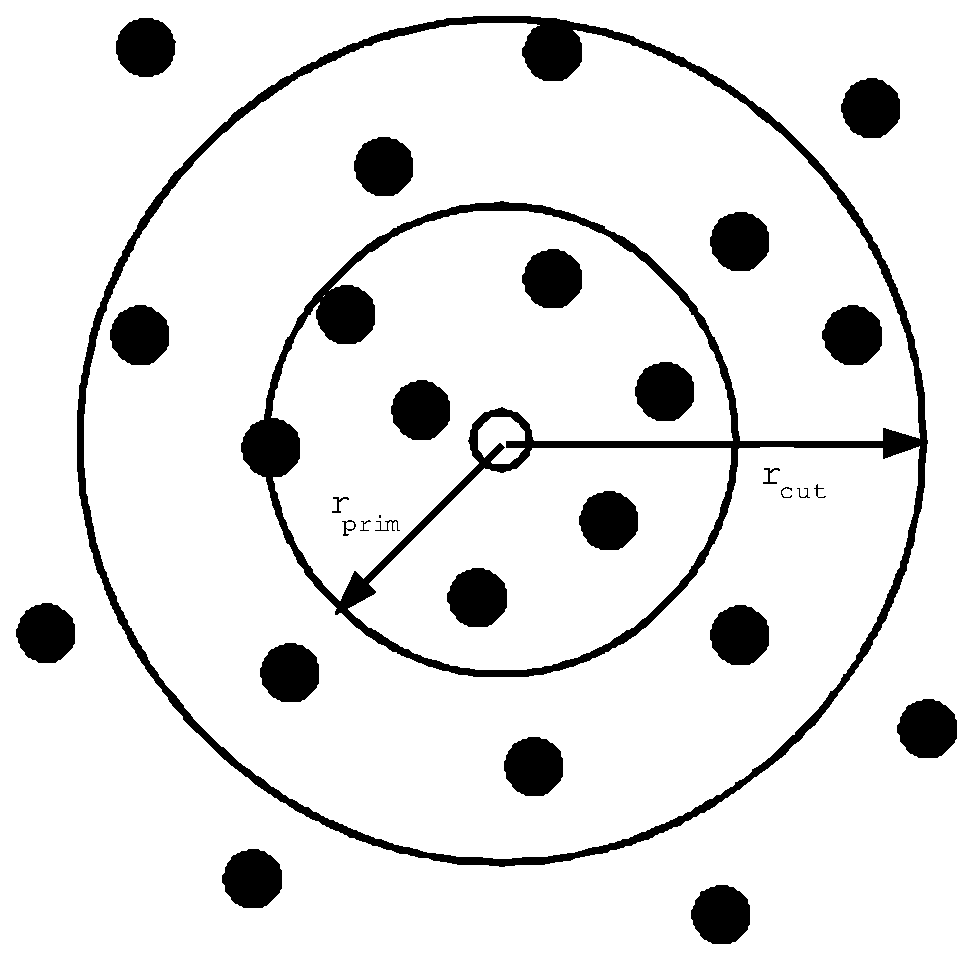
\includegraphics[height=7cm]{multi.eps}
\caption{The multiple timestep algorithm}
\end{center}
The atoms surrounding the central atom (open circle) are classified as
primary if they occur within a radius $r_{prim}$ and secondary if
outside this radius but within $r_{cut}$. Interactions arising from
primary atoms are evaluated every timestep\index{algorithm!multiple
timestep}. Interactions from secondary atoms are calculated exactly
for the first two steps of a multi-step and by extrapolation
afterwards.
\end{figure}


